\documentclass{beamer}

\usepackage[utf8]{inputenc}
\usepackage[T1]{fontenc}
\usepackage[english,russian]{babel}
\usepackage{amsmath}
\usepackage{amsfonts}
\usepackage{amssymb}
\usepackage{graphicx,pgf}
\usepackage{multimedia}
\DeclareMathOperator{\tr}{tr}
\usepackage{multirow}
\usepackage{subcaption}
\usepackage{float}


%\usetheme{Copenhagen}
\usetheme{Warsaw}
\useinnertheme{circles}   %внутренняя тема
%\useoutertheme{smoothbars}   %внешняя тема
\usecolortheme{seahorse}     %цветовая схема
%\usefonttheme{serif}    %шрифты
%\defbeamertemplate*{footline}{shadow theme}
%\setbeameroption{hide notes}

%номера слайдов
\newcommand*\oldmacro{}%
\let\oldmacro\insertshorttitle%
\renewcommand*\insertshorttitle{%
	\oldmacro\hfill%
	\insertframenumber\,/\,\inserttotalframenumber}
\RequirePackage{caption}
\DeclareCaptionLabelSeparator{defffis}{ }
\captionsetup{justification=centering,labelsep=defffis}

%\title{Курсовая работа}
%\subtitle{Численные схемы для аппроксимации неограниченных решений при моделировании обтекания профиля крыла в вихревых методах}
\title[Численное моделирование ...]{Численное моделирование напряженно-деформированного состояния твердого тела}
\author[Швецов Г.А.]{Докладчик: Швецов Г.А.\and\\[0.5mm] Научный руководитель: д.ф-м.н., профессор кафедры ФН-2 Галанин М.П.}

\institute[каф. Прикладная математика ФН-2]{группа ФН2-62Б}
\date{\today}
\titlegraphic{
\includegraphics[width=1.2cm]{logo.png}}
%\renewcommand{\vec}[1]{\text{\mathversion{bold}${#1}$}}

\begin{document}
	\newcommand{\pl}{\partial}
	\begin{frame}
		\titlepage
	\end{frame}
	
	\begin{frame}{Постановка задачи. Цель}
		\begin{block}{Цель}
			Цель работы -- рассмотрение плоской задачи термоупругости с помощью конечно-элементного алгоритма для нахождения решения на треугольной сетке, а также графическое представление результатов.
		\end{block}
		\begin{block}{Постановка задачи}
			\footnotesize
			Уравнения равновесия и матрица упругих коэффициентов
				\[
				\begin{cases}
				\dfrac{\pl\sigma_{xx}}{\pl x}+\dfrac{\pl\sigma_{yx}}{\pl y} + b_x = 0,\\
				\dfrac{\pl\sigma_{xy}}{\pl x}+\dfrac{\pl\sigma_{yy}}{\pl y} + b_y =0.						
				\end{cases}
				\]
				\[
				C=
				\begin{pmatrix}
					\lambda + 2\mu & \lambda &  0 \\
					\lambda & \lambda + 2\mu & 0 \\
					0 &      0 &       \mu \\
				\end{pmatrix}, \quad\lambda = \frac{E\nu}{(1+\nu)(1-2\nu)},\quad\mu=\frac{E}{2(1+\nu)},	
				\]
				где $E$ --- модуль Юнга, $\nu$ --- коэффициент Пуассона.
		\end{block}
	\end{frame}

\begin{frame}{Конечноэлементная постановка}
	\begin{block}{МКЭ на треугольной равномерной сетке}
	\[[K]\{U\}=R_U(T),\]
	\begin{equation*}
		\begin{cases}
			u_x=\sum\limits_{p=1}^N\sum\limits_{m=1}^3 u_{pm}^{(x)}\phi_{pm},\\
			u_y=\sum\limits_{p=1}^N\sum\limits_{m=1}^3 u_{pm}^{(y)}\phi_{pm}.
		\end{cases}
	\end{equation*}
	\end{block}
\begin{columns}
	\column{0.6\textwidth}
	\centering
	\begin{figure}[H]
	\centering
	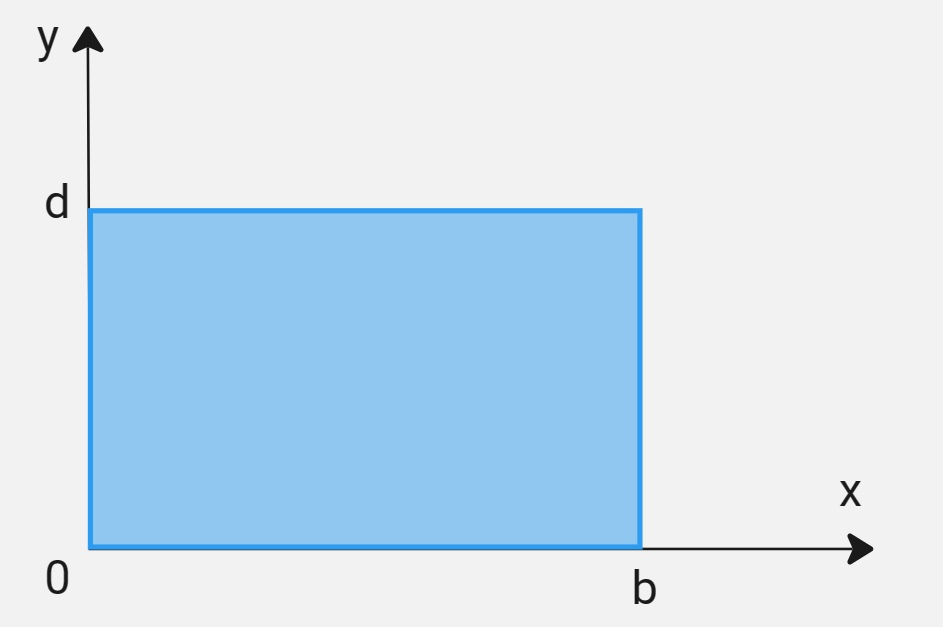
\includegraphics[width=0.8\textwidth]{p1}
\end{figure}
	\column{0.4\textwidth}
	\centering
\begin{block}{Тестовый расчет}
Пластинка обладает свойствами диоксида урана UO$_2$ и ее размеры:
\[
	b = 8 \text{ мм},\;d = 8 \text{ мм}.
\]
\end{block}
\end{columns}
\end{frame}

\begin{frame}{Порядок сходимости}	\small
\begin{block}{$\Delta T(x,y) = -1000\sqrt{\left(x-\frac{b}{2}\right)^2+\left(y-\frac{d}{2}\right)^2}$}
	\begin{tabular}{|c|c|c|c|c|}
		\hline
			Кол-во гран. узлов: & AbsErr$_{C}$ & $\Delta_C$ & AbsErr$_{L_2}$ & $\Delta_{L_2}$ \\ 
		\hline
		\multicolumn{5}{|c|}{$\mathbf{u} = \left(e^{x^2+y^2}\,;\,\tanh(xy)\right)$}\\
		\hline
	 16&7.7783e-08&3.6629&3.7796e-08&3.8817\\
	 	 32&2.0339e-08& 3.8244&1.0721e-08 &3.5255\\
	 	 	 64&6.3894e-09&3.6139&3.2510e-09 &3.6250\\
	 	 	 \hline
	 	 	 \multicolumn{5}{|c|}{$\mathbf{u} = \left(y^2e^x\,;\,\cos(xy)+\sin(xy)\right)$}\\
	 	 	 \hline
	 	 	 16&9.9139e-08&3.2458&4.9698e-08&3.7077\\
	 	 	 32&2.3091e-08&4.2934&1.1785e-08 &4.2170\\
	 	 	 64&6.3894e-09&3.6139&3.2510e-09 &3.6320\\
	 	 	 \hline
	\end{tabular}
\end{block}
Приведены ошибки в нормах $\|.\|_C$ и $\|.\|_{L_2}$, AbsErr --- абсолютная ошибка, $\Delta$ --- модуль отношения ошибок на двух соседних сетках.
\end{frame}

\begin{frame}{Линейная (несвязная) термоупругая задача}
	\begin{block}{Уравнение теплопроводности}
		\[
		\rho c_\varepsilon\frac{\pl T}{\pl t}=\mathrm{div}(\lambda\,\mathrm{grad}\, T)+f
		\]		
	\end{block}
Рассмотрим стационарный режим и положим f = 0. Пусть верхняя и нижняя стороны пластинки находятся под температурой $T_{ref}=300$ К, а боковые стороны зажаты и их нагревают на $\Delta T = 100$ К.
	\begin{figure}[H]
	\centering
	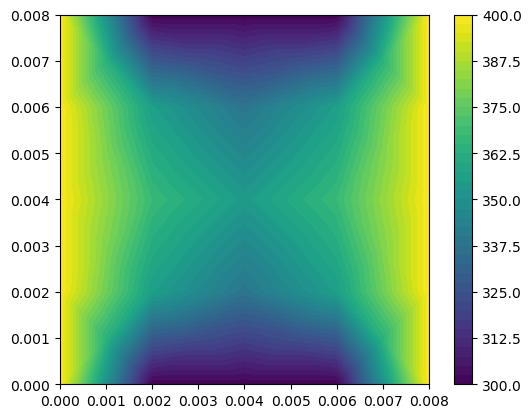
\includegraphics[width=0.5\textwidth]{tempreture1}
\end{figure}
\end{frame}

\begin{frame}{Линейная (несвязная) термоупругая задача}
\begin{figure}[H]
	\centering
	\begin{subfigure}[H]{0.4\textwidth}
		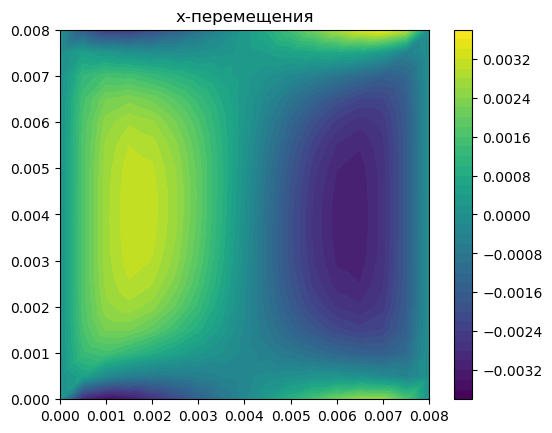
\includegraphics[width=\textwidth]{horiz1}
	\end{subfigure}
	\qquad\qquad
	\begin{subfigure}[H]{0.4\textwidth}
		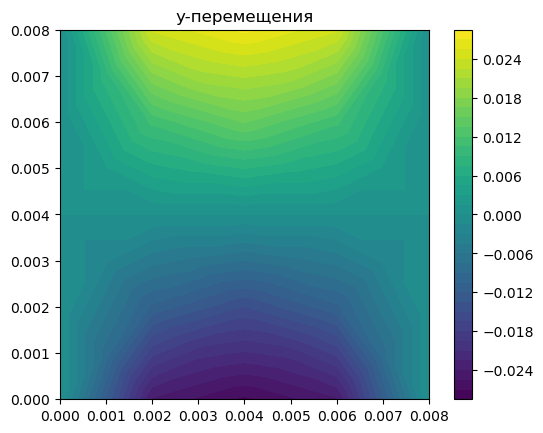
\includegraphics[width=\textwidth]{vert1}
	\end{subfigure}	
	\begin{subfigure}[H]{0.4\textwidth}
		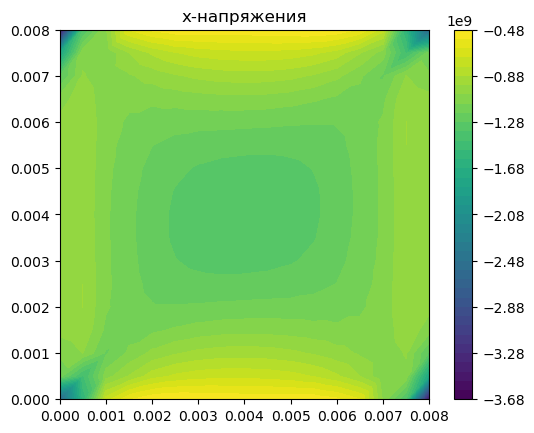
\includegraphics[width=\textwidth]{stress_x}
	\end{subfigure}
	\qquad\qquad
	\begin{subfigure}[H]{0.4\textwidth}
		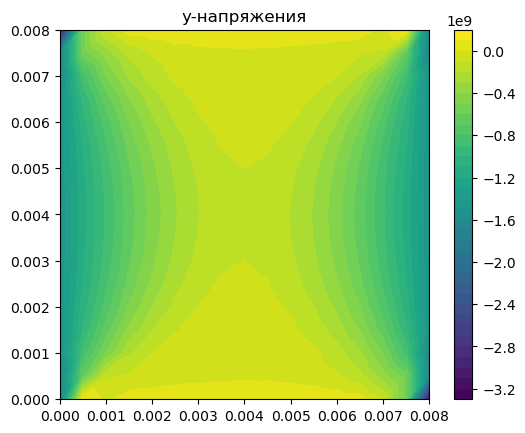
\includegraphics[width=\textwidth]{xtress_y}
	\end{subfigure}	
\end{figure}	
\end{frame}

	\begin{frame}{Модель размазанных трещин}
		\begin{block}{Аппроксимация}
			\begin{equation}
				\dfrac{\sigma}{\sigma_f} = A + B e^{-C \tfrac{\varepsilon}{\varepsilon_f}},	
			\end{equation}
			где коэффициенты A, B выводятся экспериментально.\\ Для дикосида урана UO$_2$:
			$
			A = -0.024,\, B = 1.69, \, C = 0.5.  
			$
		\end{block}
		\begin{figure}[h]
			\centering
			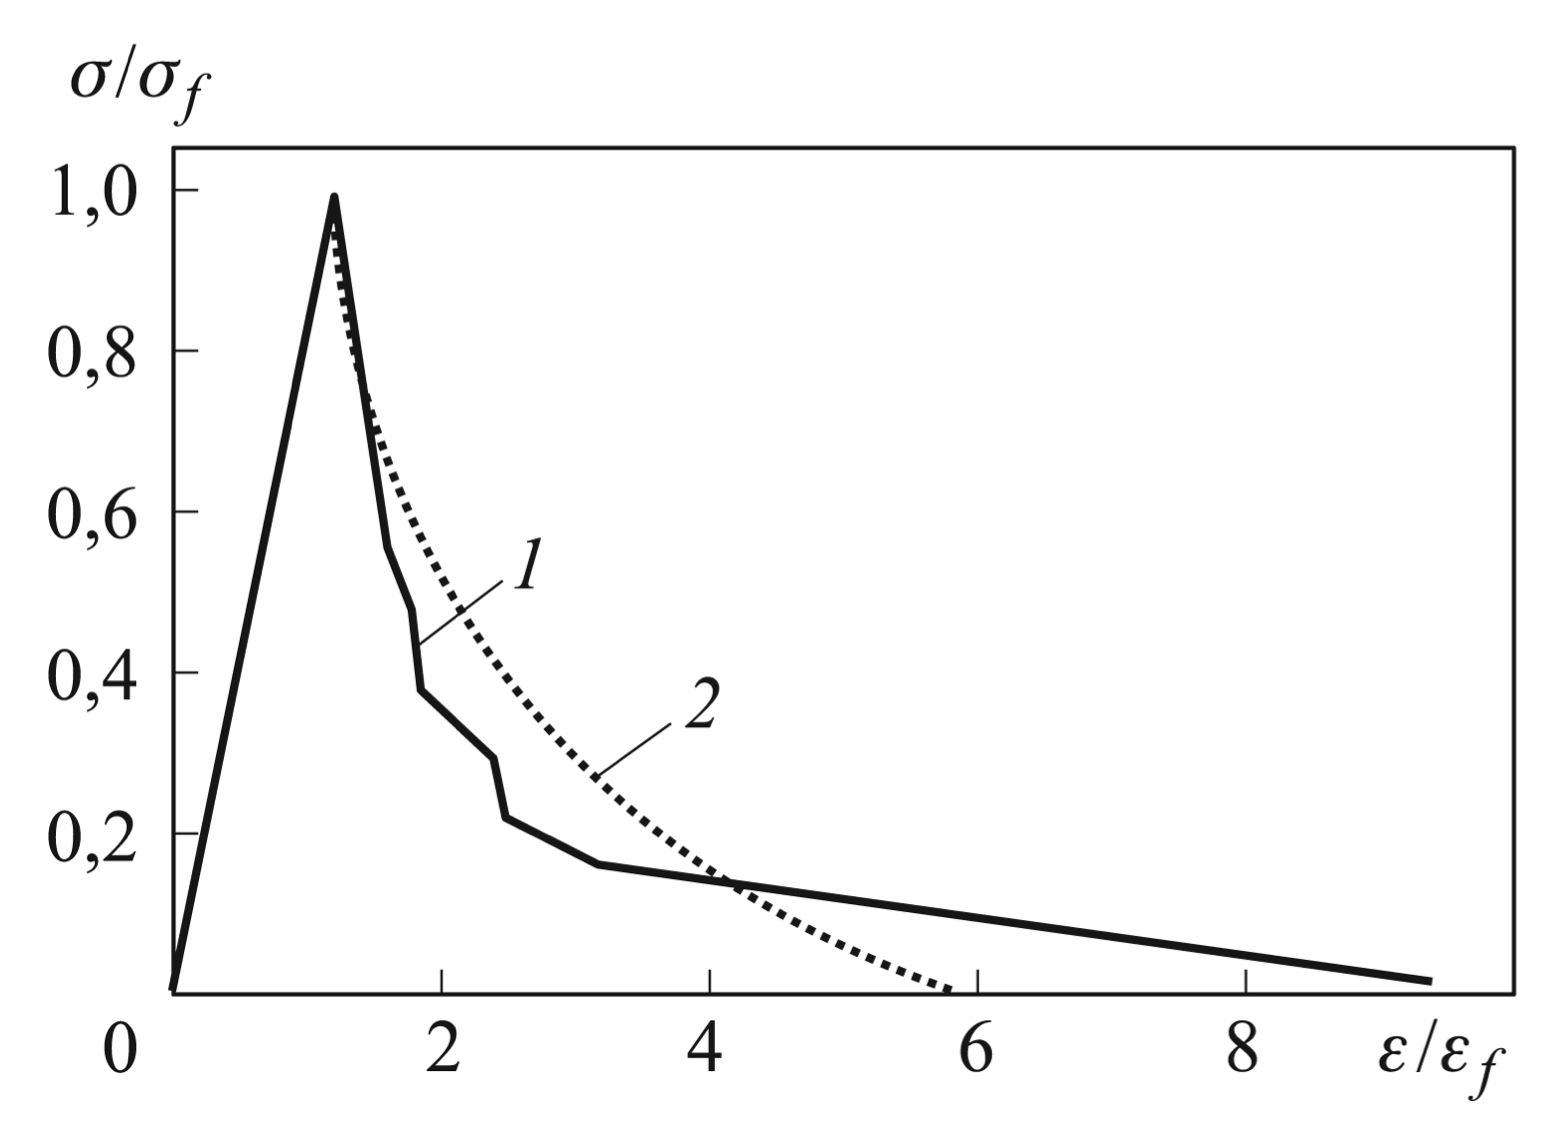
\includegraphics[width=0.53\textwidth]{ceramic}
				\captionsetup{labelformat=empty}
			\caption{\small{Экспериментальная (1) и аналитическая (2) кривые растягивающего отклика для керамических материалов}}
			%	\caption{Экспериментальная (1) и аналитическая (2) кривые нормализованного растягивающего отклика для керамических материалов}

		\end{figure}
	\end{frame}

\begin{frame}{Образование радиальных трещин}
	\begin{columns}
		\column{0.5\textwidth}
		\centering
		\begin{figure}[H]
			\centering
			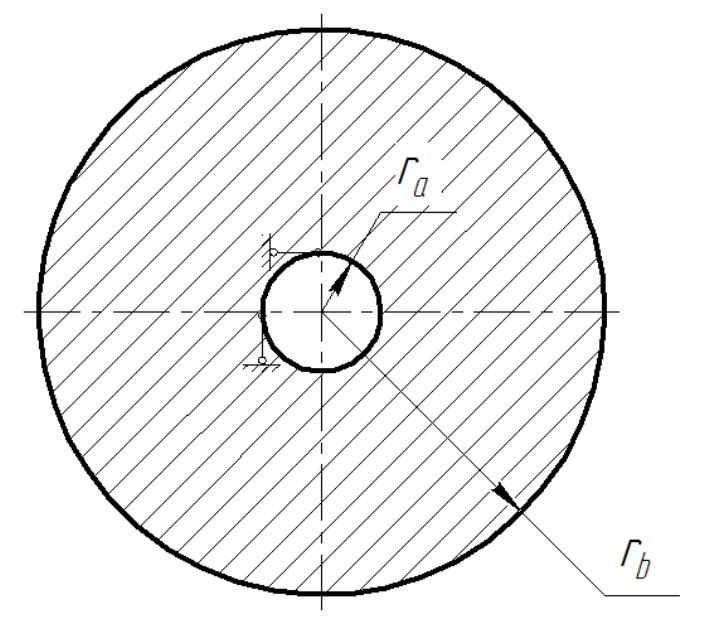
\includegraphics[width=0.8\textwidth]{crack}
		\end{figure}
		\column{0.5\textwidth}
		\centering
		\begin{block}{Тестовый расчет}
			\[
			\begin{gathered}
			r_a = 0,8 \text{ мм},\;d = 3,8 \text{ мм},\\
				u_x(0,r_a) = u_y(-r_a,0)=0,\\ \sigma_{xx}\left.\right|_{x^2+y^2=r_a^2}=0,\\\sigma_{yy}\left.\right|_{x^2+y^2=r_b^2}=0,
				t_f=1 \text{ c}.
			\end{gathered}
			\]
		\end{block}
	\end{columns}
\begin{block}{Температура}
	\[
	\begin{gathered}
	T(x,y,t)=\frac{T_1(t)\ln\dfrac{r_b}{r}-T_2(t)\ln\dfrac{r_a}{r}}{\ln\dfrac{r_b}{r_a}}, \\
	T_1(t)=(T_a-T_0)\frac{t}{t_f}+T_0,\;T_2(t)=(T_b-T_0)\frac{t}{t_f}+T_0,\\T_a = 1700 \text{ K},\;T_b = 600 \text{ K},\;T_0=T_{ref}
	\end{gathered}
	\]
\end{block}	
\end{frame}
	
	\begin{frame}{$\sigma_{xx}(x,y),\,\sigma_{yy}(x,y)$ при $t = 0.06t_f,\,t=0.2t_f$}
\begin{figure}[H]
\centering
\begin{subfigure}[H]{0.4\textwidth}
	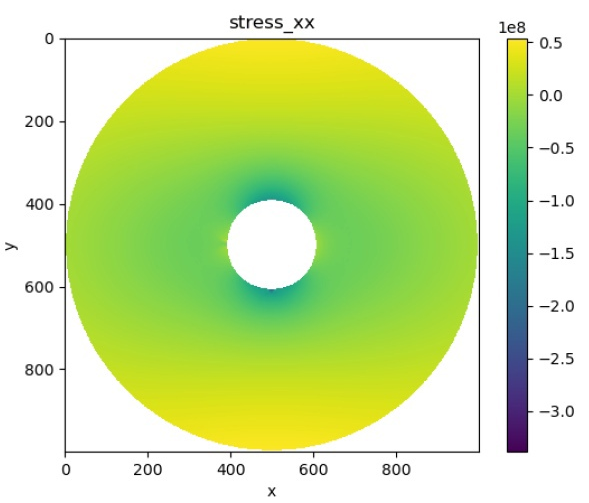
\includegraphics[width=\textwidth]{stressx_06tf}
\end{subfigure}
\qquad\qquad
\begin{subfigure}[H]{0.4\textwidth}
	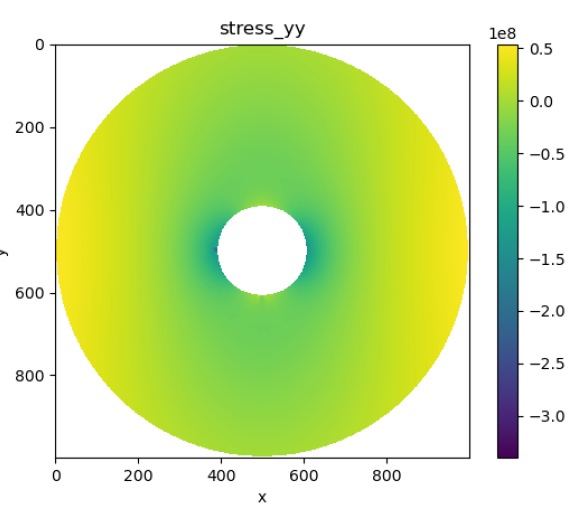
\includegraphics[width=\textwidth]{stressy_06tf}
\end{subfigure}	
\begin{subfigure}[H]{0.4\textwidth}
	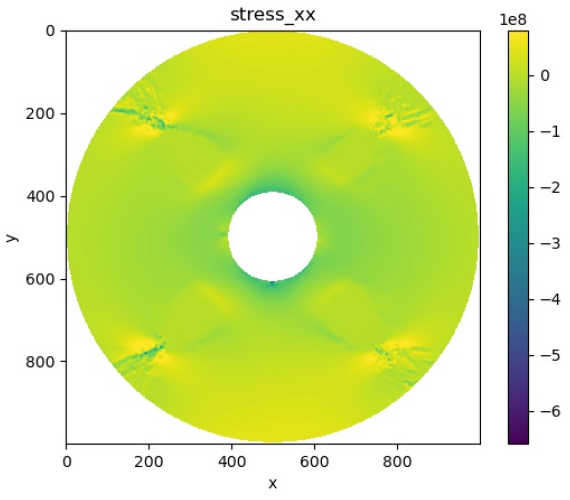
\includegraphics[width=\textwidth]{stressx_002}
\end{subfigure}
\qquad\qquad
\begin{subfigure}[H]{0.4\textwidth}
	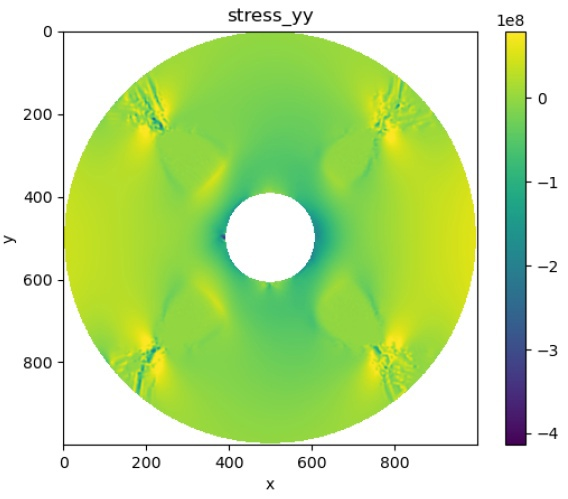
\includegraphics[width=\textwidth]{stressy_002}
\end{subfigure}	
\end{figure}	
	\end{frame}

	\begin{frame}{$\sigma_{xx}(x,y),\,\sigma_{yy}(x,y)$ при $t = 0.9t_f,\,t=t_f$}
	\begin{figure}[H]
		\centering
		\begin{subfigure}[H]{0.4\textwidth}
			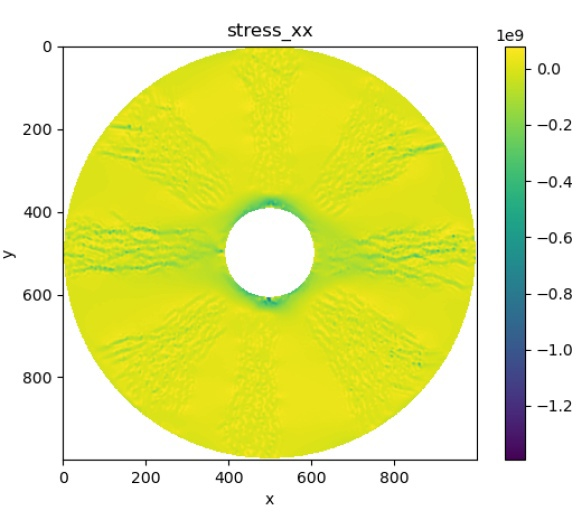
\includegraphics[width=\textwidth]{stressx_2tf}
		\end{subfigure}
		\qquad\qquad
		\begin{subfigure}[H]{0.4\textwidth}
			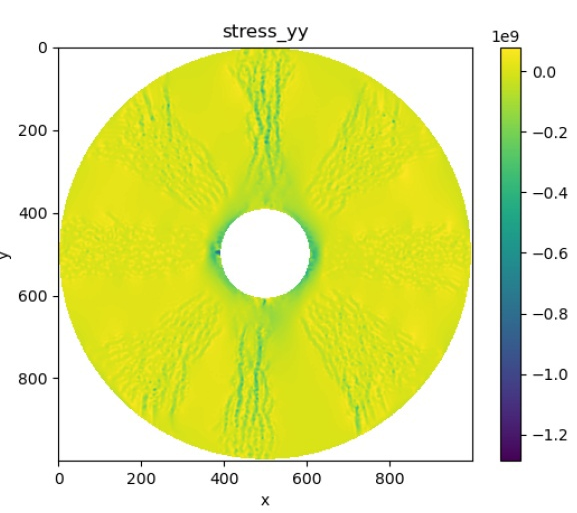
\includegraphics[width=\textwidth]{stressy_2tf}
		\end{subfigure}	
		\begin{subfigure}[H]{0.4\textwidth}
		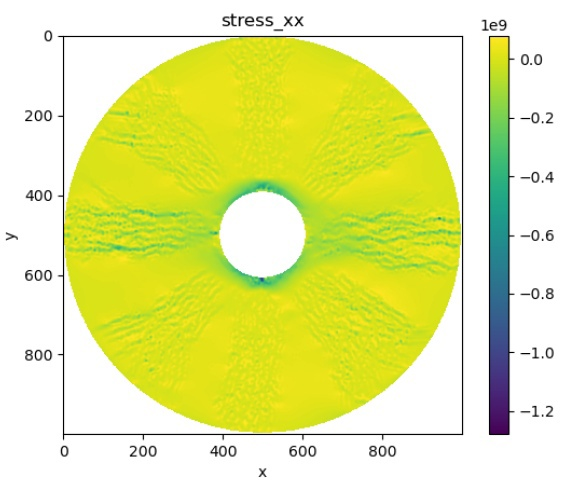
\includegraphics[width=\textwidth]{stressx_tf}
	\end{subfigure}
	\qquad\qquad
	\begin{subfigure}[H]{0.4\textwidth}
		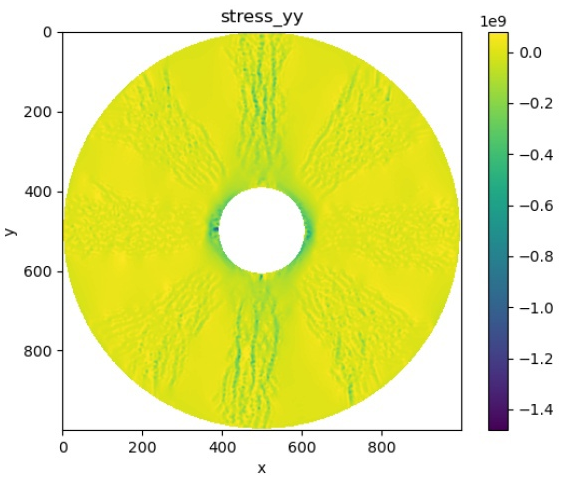
\includegraphics[width=\textwidth]{stressy_tf}
	\end{subfigure}	
	\end{figure}	
\end{frame}

\begin{frame}{Минимум функции памяти $e_{min} = \min(e_1,e_2)$}
\begin{figure}[H]
	\centering
	\begin{subfigure}[H]{0.4\textwidth}
		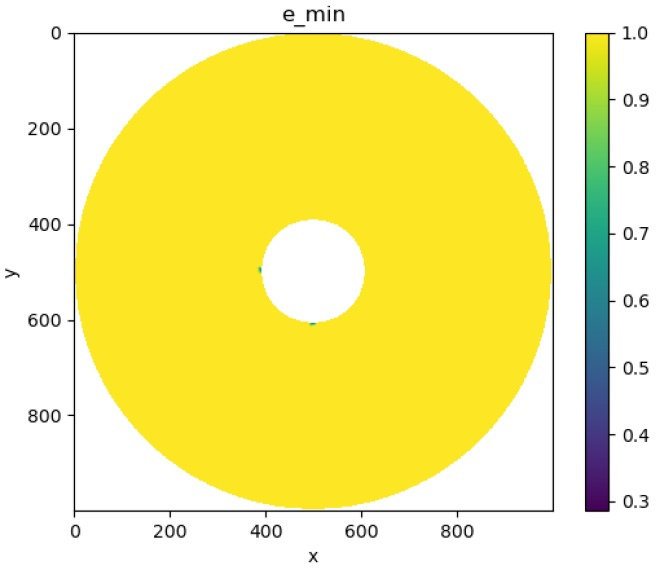
\includegraphics[width=\textwidth]{e_06tf}
	\end{subfigure}
	\qquad\qquad
	\begin{subfigure}[H]{0.4\textwidth}
		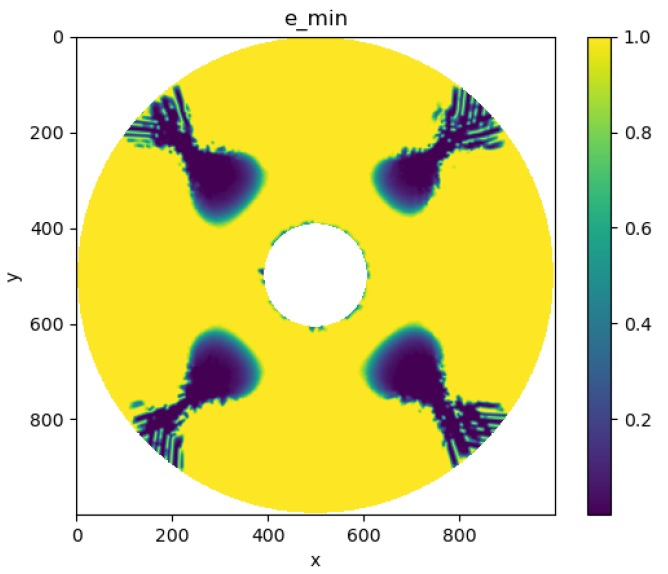
\includegraphics[width=\textwidth]{e_002}
	\end{subfigure}	
	\begin{subfigure}[H]{0.4\textwidth}
		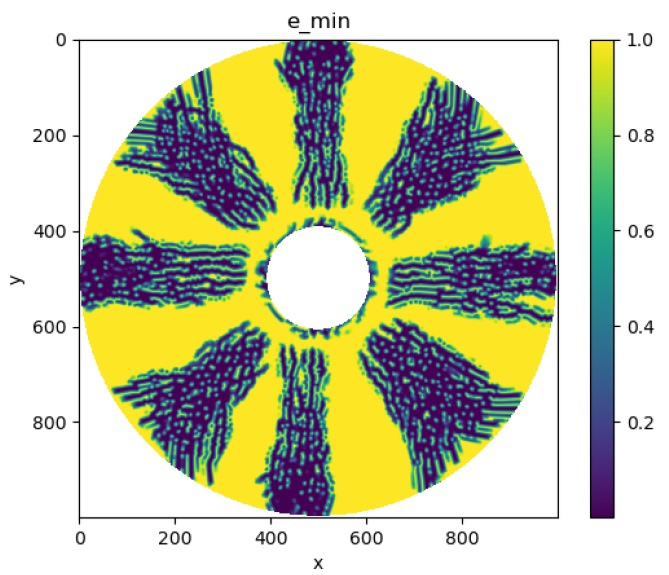
\includegraphics[width=\textwidth]{e_2tf}
	\end{subfigure}
	\qquad\qquad
	\begin{subfigure}[H]{0.4\textwidth}
		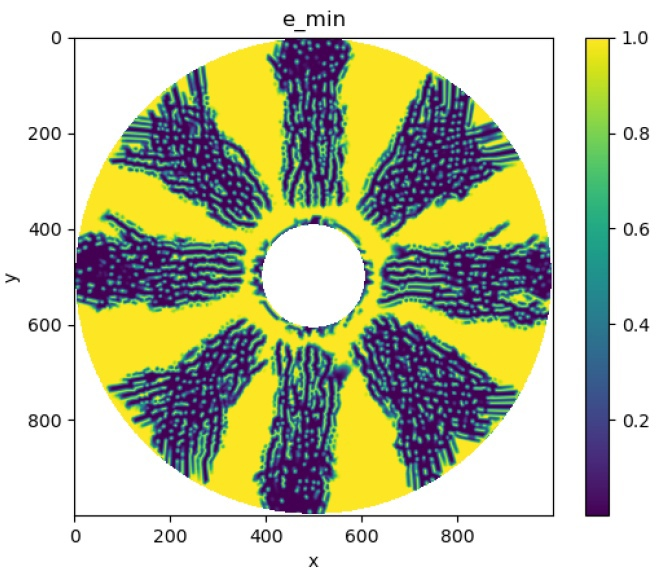
\includegraphics[width=\textwidth]{e_tf}
	\end{subfigure}	
\end{figure}		
\end{frame}
	
	
	\begin{frame}{Заключение}
		\large
		\begin{enumerate}
			\item Методом конечных элементов на равномерной сетке решена задача термоупругости;
			\item Найден порядок точности схемы для тестовых задач;
			\item Проведено математическое моделирование разрушения топливной таблетки в двумерной задаче;
			\item Проведен графический анализ распространения трещин, основанный на графиках напряжений в различные промежутки времени.
		\end{enumerate}
	\end{frame}
	
	
	\begin{frame}
		\frametitle{Список использованных источников}
		\begin{thebibliography}{9}
			
			\bibitem{galanin1} \textit{Галанин М.П., Савенков Е.Б.} Методы численного анализа математических моделей. М.: Изд-во МГТУ им. \mbox{Н.Э. Баумана},	2010. -- 592 с.
			
			\bibitem{galanin2} Математическое моделирование разрушения хрупкого материала под действием тепловых нагрузок / М.П. Галанин [и др.] // Препринты ИПМ им. М.В. Келдыша. 2013.No 100. -- 36 с. URL: \url{http://library.keldysh.ru/preprint.asp?id=2013-100}
			
			\bibitem{frost} \textit{Фрост Б.} ТВЭЛы ядерных реакторов: пер. с англ. М.: Энергоатомиздат, 1986. --
			\mbox{248 с.}
			\bibitem{zarubin} \textit{Зарубин В.С., Кувыркин Г.Н.} Математические модели механики и электродинамики сплошной среды. -- М.: Изд-во МГТУ им. Н.Э. Баумана, 2008. -- 512 с.: ил. (Математическое моделирование в технике и в технологии).
			
		\end{thebibliography}
	\end{frame}
	
	\begin{frame}
		\LARGE
		\centering
		Спасибо за внимание!
	\end{frame}
	
	
	
\end{document}